
\begin{frame}{目录}
        \begin{center}
            \textcolor{NJU_purple}{\Large 第一部分} \\
            \text{\;} \\
            \textcolor{NJU_purple}{\Huge GRU的提出背景} 
        \end{center}      
    \end{frame}

\begin{frame}{背景1:RNN的局限性}
    \begin{itemize}
        \item RNN的核心原理
        \begin{equation*}
            h_t = f_W(h_{t-1}, x_t)
        \end{equation*}
        \begin{itemize}
            \item 即对于每个时间步,隐藏层的净输入\(z_t = Uh_{t-1} + W x_{t} + b\)
            \item 隐藏层的状态为\(h_t = f(z_t)\),其中\(f\)为非线性激活函数。
        \end{itemize}
        \item 更新参数:时间反向传播(BPTT)
        \begin{itemize}
            \item 损失函数为\(L_t\),定义误差项\(\sigma_{t,k} = \frac{\partial L_t}{\partial z_k}\)为第\(t\)时刻损失对第\(k\)时刻隐藏神经层净输入的导数,即
            \begin{equation*}
                \sigma_{t,k} = \frac{\partial L_t}{\partial z_k} = \frac{\partial h_k}{\partial z_k} \frac{\partial z_{k + 1}}{\partial h_k} \frac{\partial L_t}{\partial z_{k + 1}} = diag(f'(z_k))U^T \sigma_{t,k+1}
            \end{equation*}
            \item 整个序列的损失函数\(L\)关于参数\(U\),权重\(W\)和偏置\(b\)的梯度分别为
            \begin{equation*}
                \frac{\partial L}{\partial U} = \sum_{t=1}^{T}\sum_{k=1}^t\sigma_{t,k}h_{k-1}^T \quad \frac{\partial L}{\partial W} = \sum_{t=1}^{T}\sum_{k=1}^t\sigma_{t,k}x_k^T \quad \frac{\partial L}{\partial b} = \sum_{t=1}^{T}\sum_{k=1}^t\sigma_{t,k}
            \end{equation*}
        \end{itemize}
        \end{itemize}
\end{frame}

\begin{frame}{背景1:RNN的局限性}
    \begin{itemize}
        \item 梯度爆炸或消失:RNN通过时间反向传播(BPTT)更新参数时,梯度会随着时间步呈指数级衰减或爆炸,导致远距离依赖难以捕捉。
        \begin{itemize}
            \item 梯度爆炸:当\(diag(f'(z_k))U^T > 1\)时,如果时间间隔过大,\(\sigma_{t,k}\)会趋向无穷,产生梯度爆炸问题
            \item 梯度消失:当\(diag(f'(z_k))U^T < 1\)时,如果时间间隔过大,\(\sigma_{t,k}\)会趋向0,产生梯度消失问题
        \end{itemize}
        \item 记忆容量有限:RNN的隐藏状态(Hidden State)需同时承担“记忆历史信息”和“生成当前输出”的双重任务,难以长期保留关键信息。
    \end{itemize}
\end{frame}

\begin{frame}{背景2:LSTM的局限性}
    \begin{itemize}
        \item LSTM采用两大机制解决RNN的缺点
        \begin{itemize}
            \item 梯度消失或爆炸的问题:采用门控机制(输入门、遗忘门、输出门)解决
            \begin{itemize}
                \item 遗忘门:\(f_t = \sigma(W_f \cdot [h_{t-1}, x_t] + b_f)\)
                \item 输入门:\(i_t = \sigma(W_i \cdot [h_{t-1}, x_t] + b_i)\)
                \item 输出门:\(o_t = \sigma(W_o \cdot [h_{t-1}, x_t] + b_o)\)
            \end{itemize}
            \item 短期记忆覆盖长期记忆的问题:采用记忆单元(Cell State)来保存长期记忆
            \begin{itemize}
                \item 记忆的更新:\(\tilde{c}_t = \tanh(W_c \cdot [h_{t-1}, x_t] + b_c) \quad  c_t = f_t * c_{t-1} + i_t * \tilde{c}_t\)
            \end{itemize}
        \end{itemize}
    \end{itemize}
\end{frame}

\begin{frame}{背景2:LSTM的局限性}
    \begin{figure}
        \centering
        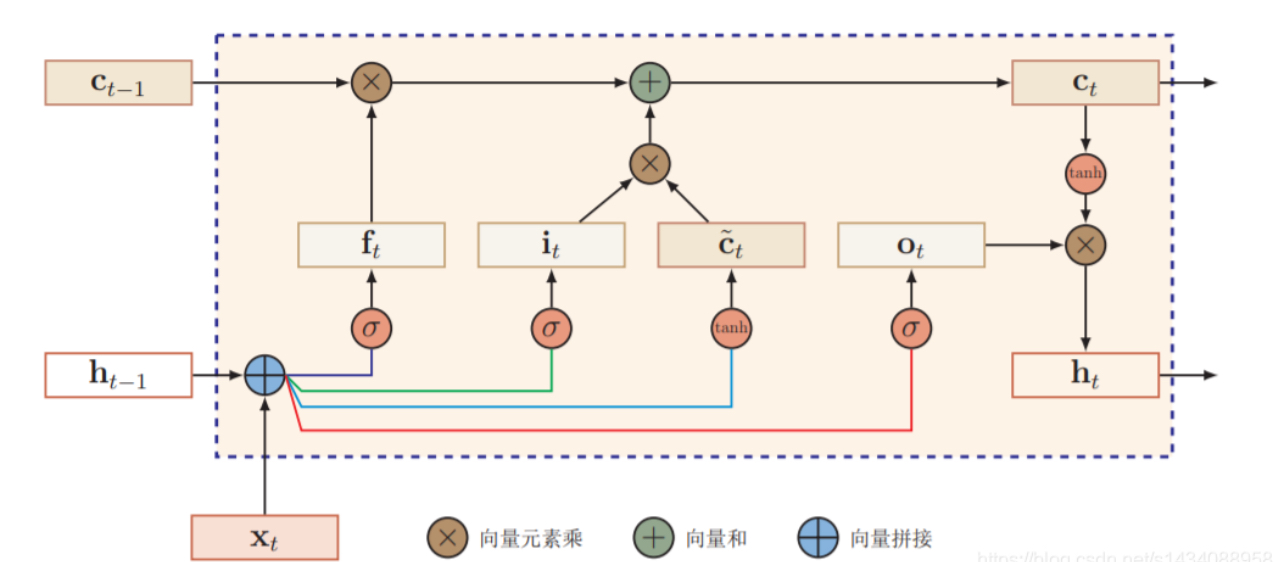
\includegraphics[width=0.65\linewidth]{pic/LSTM原理图.png}
        \caption{LSTM原理图}
        \label{fig:LSTM}
    \end{figure}
    \begin{itemize}
        \item LSTM解决了梯度问题,但结构复杂。
        \begin{itemize}
            \item 参数量大:LSTM包含3个门控和1个记忆单元,计算复杂度高。
            \item 训练效率低:复杂的结构导致训练速度较慢,尤其在长序列场景下。
        \end{itemize}
    \end{itemize}
\end{frame}





